\subsection[The Aho-Corasick algorithm]{The Aho-Corasick algorithm}
    \subsubsection{Introduction \& Application}
        \begin{itemize}
            \item \textbf{Core idea:} According to Abdeen\cite{abdeen2011algorithm}, the brute-force algorithm works with two pointers; a "text pointer" i
        and a "pattern pointer" j. For all possible shifts of the pattern P over the text T,
        compare the pattern characters with the corresponding text characters.
        If mismatch occurs, i is incremented by 1, and j is reset to 0 and the comparing
        process is restarted. In the case that all characters match, the algorithm records
        the position of the match and continues searching for the next possible match.
            \item \textbf{Real-world applications:}
            \begin{itemize}
                \item Text Editors: Using in "Search" or "Find and Replace" features to locate destination words.
                \item Bioinformatics: Searching for specific DNA.
                \item Checking for Plagiarism: Comparing documents to find and compare a script or a piece of code with the exact match in a large database.
            \end{itemize}
        \end{itemize}

    \subsubsection{Pseudocode}
        \textbf{Notation:}
        \begin{itemize}
            \item \textbf{Trie Node}: A structure containing a character $pC$, a list of pattern indices $pos$, child pointers $nxt$, transition pointers $go$, a suffix link $link$, and a parent pointer $par$.
            \item \textbf{Text $T$ (R rows, C columns)}: The 2D grid of characters.
            \item \textbf{Pattern $P$ (K keywords)}: The list of patterns to search for.
            \item \textbf{List\_string}: A 1D array of size $M = R + C$, containing all rows followed by all columns extracted from $T$.
        \end{itemize}

        \textsc{Add-String}($S, idx, root$)
        \begin{algorithmic}[1]
        \State $cur = root$
        \For{\textbf{each} character $c$ \textbf{in} $S$}
            \If{$cur.nxt[c] == \textbf{null}$}
                \State $cur.nxt[c] = \text{new Node}$
                \State $cur.nxt[c].par = cur$
                \State $cur.nxt[c].pC = c$
            \EndIf
            \State $cur = cur.nxt[c]$
        \EndFor
        \State \text{append } $idx$ \text{ to } $cur.pos$
        \end{algorithmic}

        \textsc{Get-Link}($u, root$)
        \begin{algorithmic}[1]
        \If{$u.link == \textbf{null}$}
            \If{$u == root$ \textbf{or} $u.par == root$}
                \State $u.link = root$
            \Else
                \State $u.link = \textsc{Go}(\textsc{Get-Link}(u.par), u.pC)$
            \EndIf
        \EndIf
        \State \Return $u.link$
        \end{algorithmic}

        \textsc{Go}($u, c, root$)
        \begin{algorithmic}[1]
        \If{$u.go[c] == \textbf{null}$}
            \If{$u.nxt[c] \neq \textbf{null}$}
                \State $u.go[c] = u.nxt[c]$
            \Else
                \State $u.go[c] = (u == root) \text{ ? } u : \textsc{Go}(\textsc{Get-Link}(u), c)$
            \EndIf
        \EndIf
        \State \Return $u.go[c]$
        \end{algorithmic}

        \textsc{Search-String}($S, IDX, R, P, ans, root$)
        \begin{algorithmic}[1]
        \State $cur = root$
        \For{$i = 0$ \textbf{to} $S.length - 1$}
            \State $cur = \textsc{Go}(cur, S[i])$
            \State $tmp = cur$
            \While{$tmp \neq root$}
                \For{\textbf{each} $idx$ \textbf{in} $tmp.pos$}
                    \State $m = P[idx].length$
                    \If{$IDX < R$} 
                        \Comment{Horizontal match (Row extraction)}
                        \State $start = (IDX, i - m + 1)$
                        \State $end = (IDX, i)$
                    \Else 
                        \Comment{Vertical match (Column extraction)}
                        \State $start = (i - m + 1, IDX - R)$
                        \State $end = (i, IDX - R)$
                    \EndIf
                    \State \text{append } $(start, end)$ \text{ to } $ans[idx]$
                \EndFor
                \State $tmp = \textsc{Get-Link}(tmp)$
            \EndWhile
        \EndFor
        \end{algorithmic}

        \textsc{Aho-Corasick}($T, P, K, R, C$)
        \begin{algorithmic}[1]
        \State $List\_string = \textsc{Convert-Grid-To-Strings}(T)$
        \State $ans = \text{array of } K \text{ empty lists}$
        \State $root = \text{new Node}$
        \State $maxLen = \max(R, C)$
        \Statex
        \Comment{Build the Trie}
        \For{$i = 0$ \textbf{to} $K - 1$}
            \If{$P[i].length \leq maxLen$}
                \State $\textsc{Add-String}(P[i], i, root)$
            \EndIf
        \EndFor
        \Statex
        \Comment{Process all rows and columns}
        \For{$i = 0$ \textbf{to} $List\_string.length - 1$}
            \State $\textsc{Search-String}(List\_string[i], i, R, P, ans, root)$
        \EndFor
        \Statex
        \State $\textsc{Remove-Trie}(root)$ \Comment{Free allocated memory}
        \State \Return $ans$
        \end{algorithmic}

    \subsubsection{Step-by-step trace\cite{CLRS2022}}
    \indent \textbf{Notation:}
        \begin{itemize}
            \item \textbf{Text $T$ (length $n$)}: The main text being searched.
            \item \textbf{Pattern $P$}: The string that we are looking for.
            \item \textbf{Shift ($s$)}: The current offset of the text T.
            \item \textbf{Positions ([(start position, end position), \ldots])}: A list storing the indices where a complete match is found.
        \end{itemize}

    \indent \textbf{Example:} text $T = [a, a, b, c, a, b, b]$ and pattern $P = [a, b, c]$
    \begin{itemize}
        \begin{figure}[H]
            \centering
            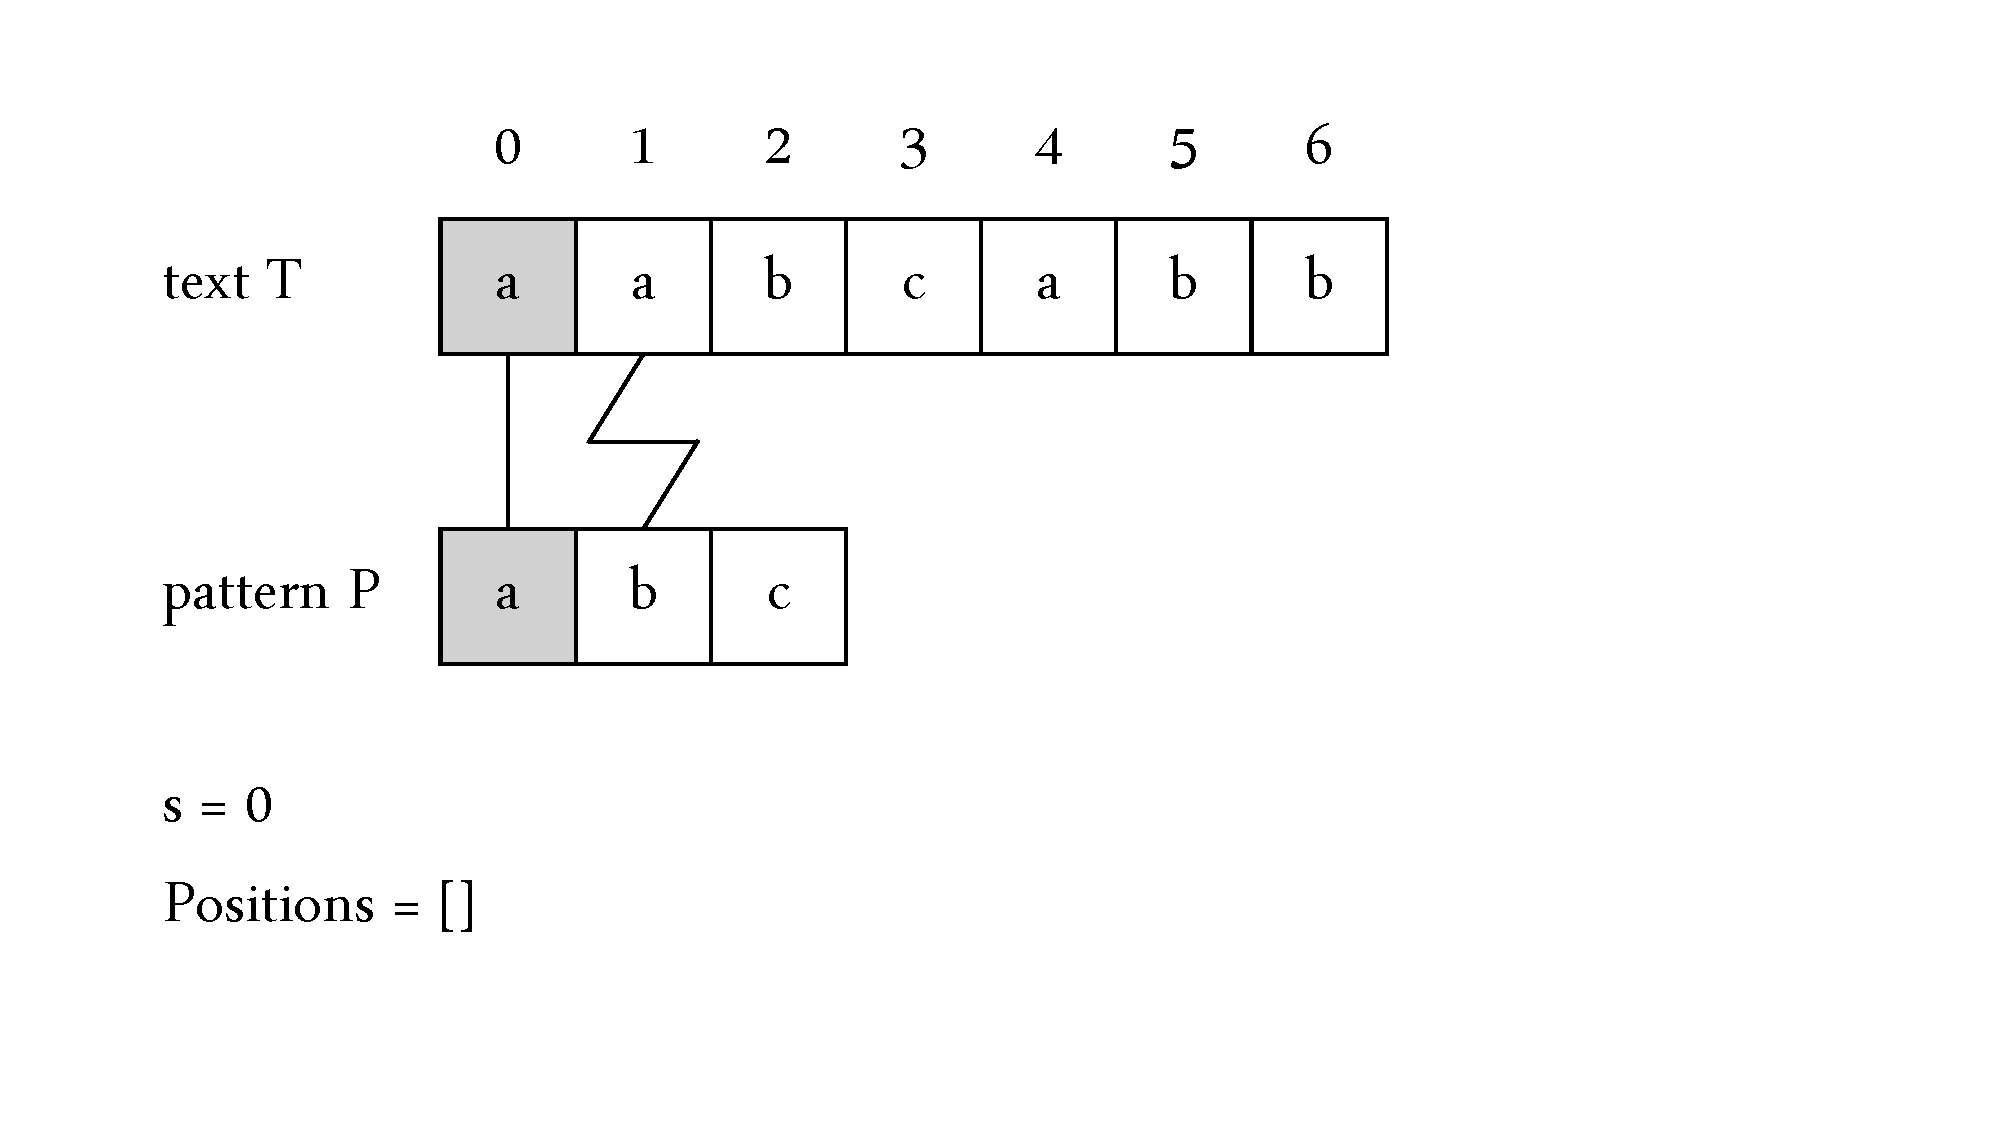
\includegraphics[width=0.8\textwidth, trim={2cm 2cm 5cm 2cm}, clip]{data/Illustrations/brute-force1.pdf}
            \caption{Step 1}
        \end{figure}
        \item The first character 'a' matches in both arrays.
        
        The second character in text $T$ ('a') does not match the second character in pattern $P$ ('b').
        
        Text at the bottom shows the current shift is $s = 0$ and the list of found matches is empty ($Positions = []$).
        
        \begin{figure}[H]
            \centering
            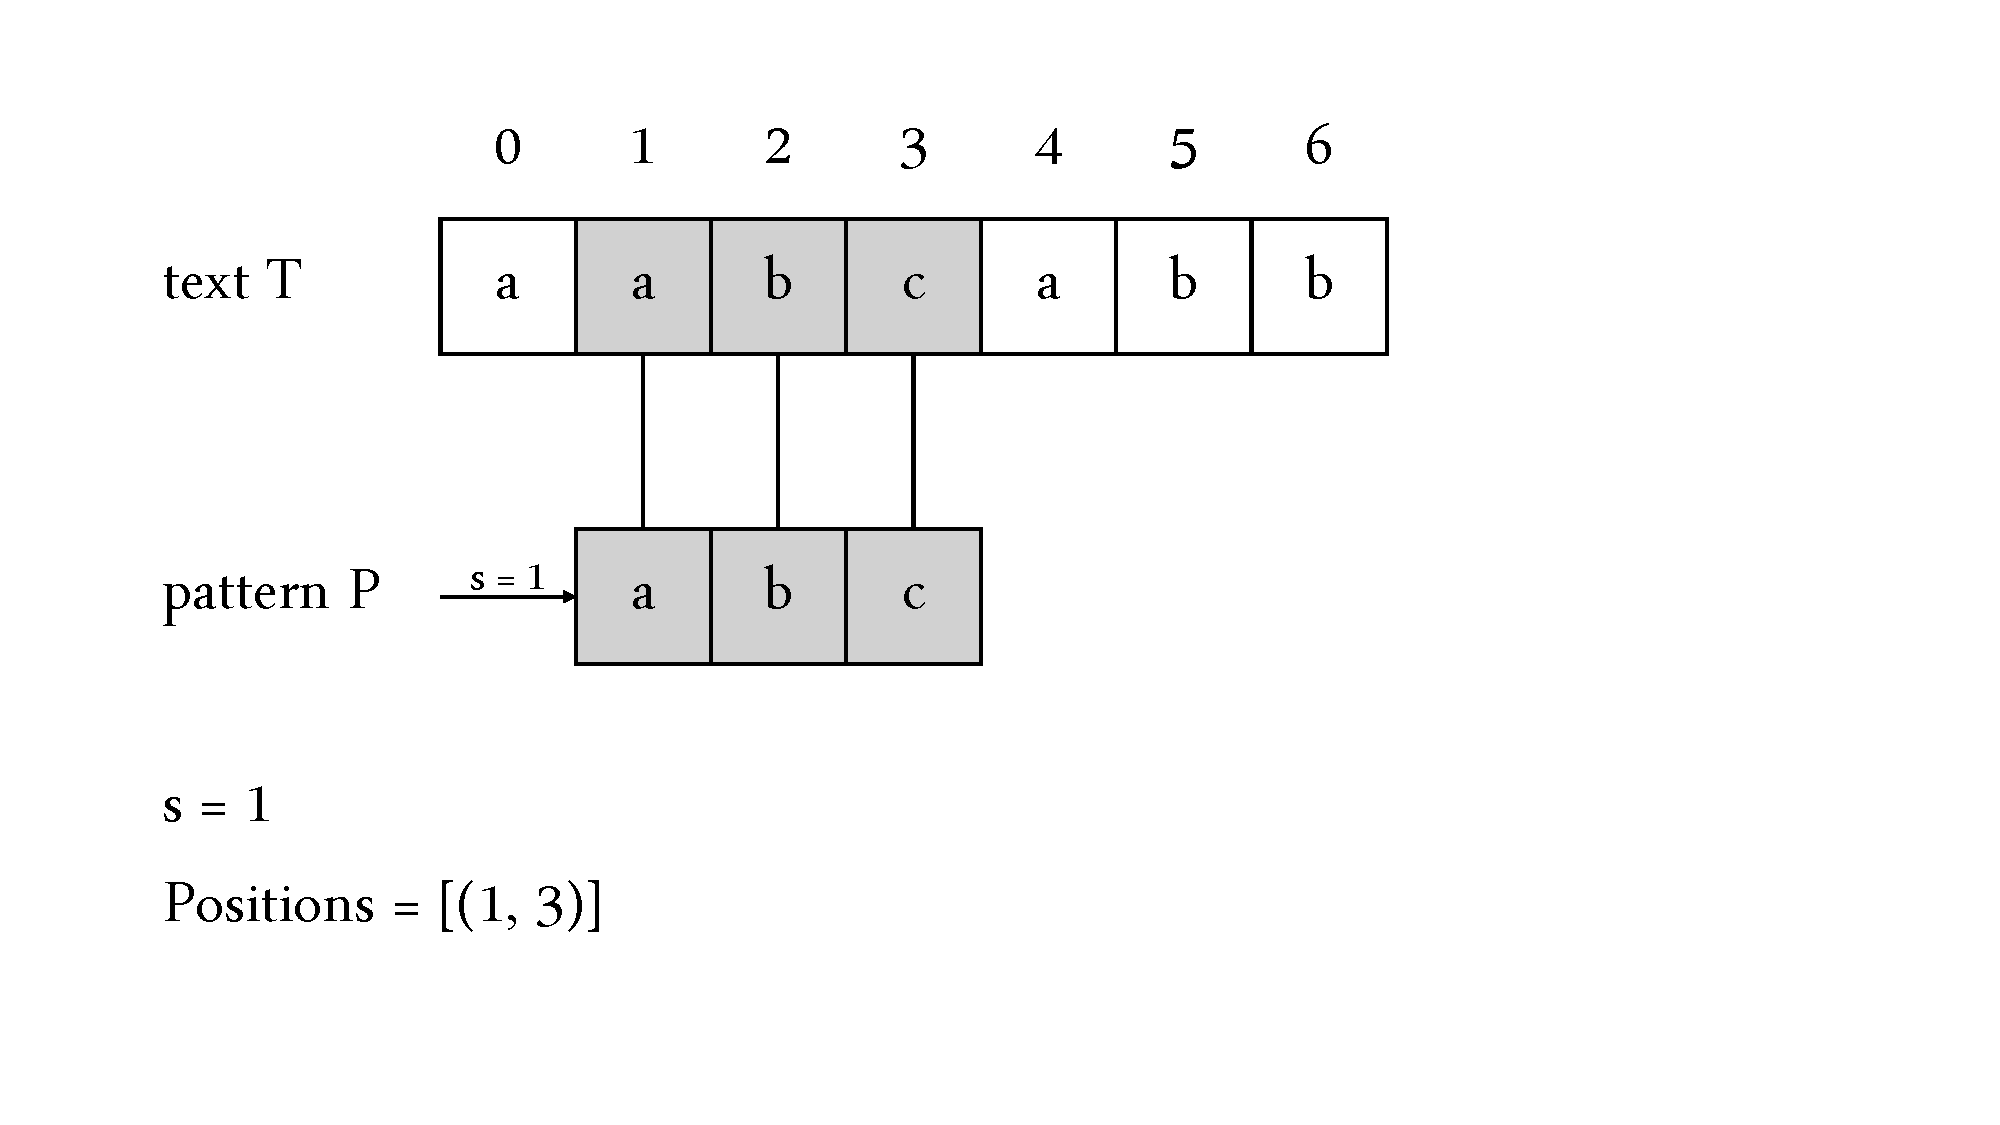
\includegraphics[width=0.8\textwidth, trim={2cm 2cm 5cm 2cm}, clip]{data/Illustrations/brute-force2.pdf}
            \caption{Step 2}
        \end{figure}
        \item All characters in pattern $P$ ('a', 'b', 'c') successfully match the corresponding characters in text $T$ ('a', 'b', 'c').
        
        Shift is $s = 1$ and the list of found matches is updated to record this position ($Positions = [(1, 3)]$).

        \begin{figure}[H]
            \centering
            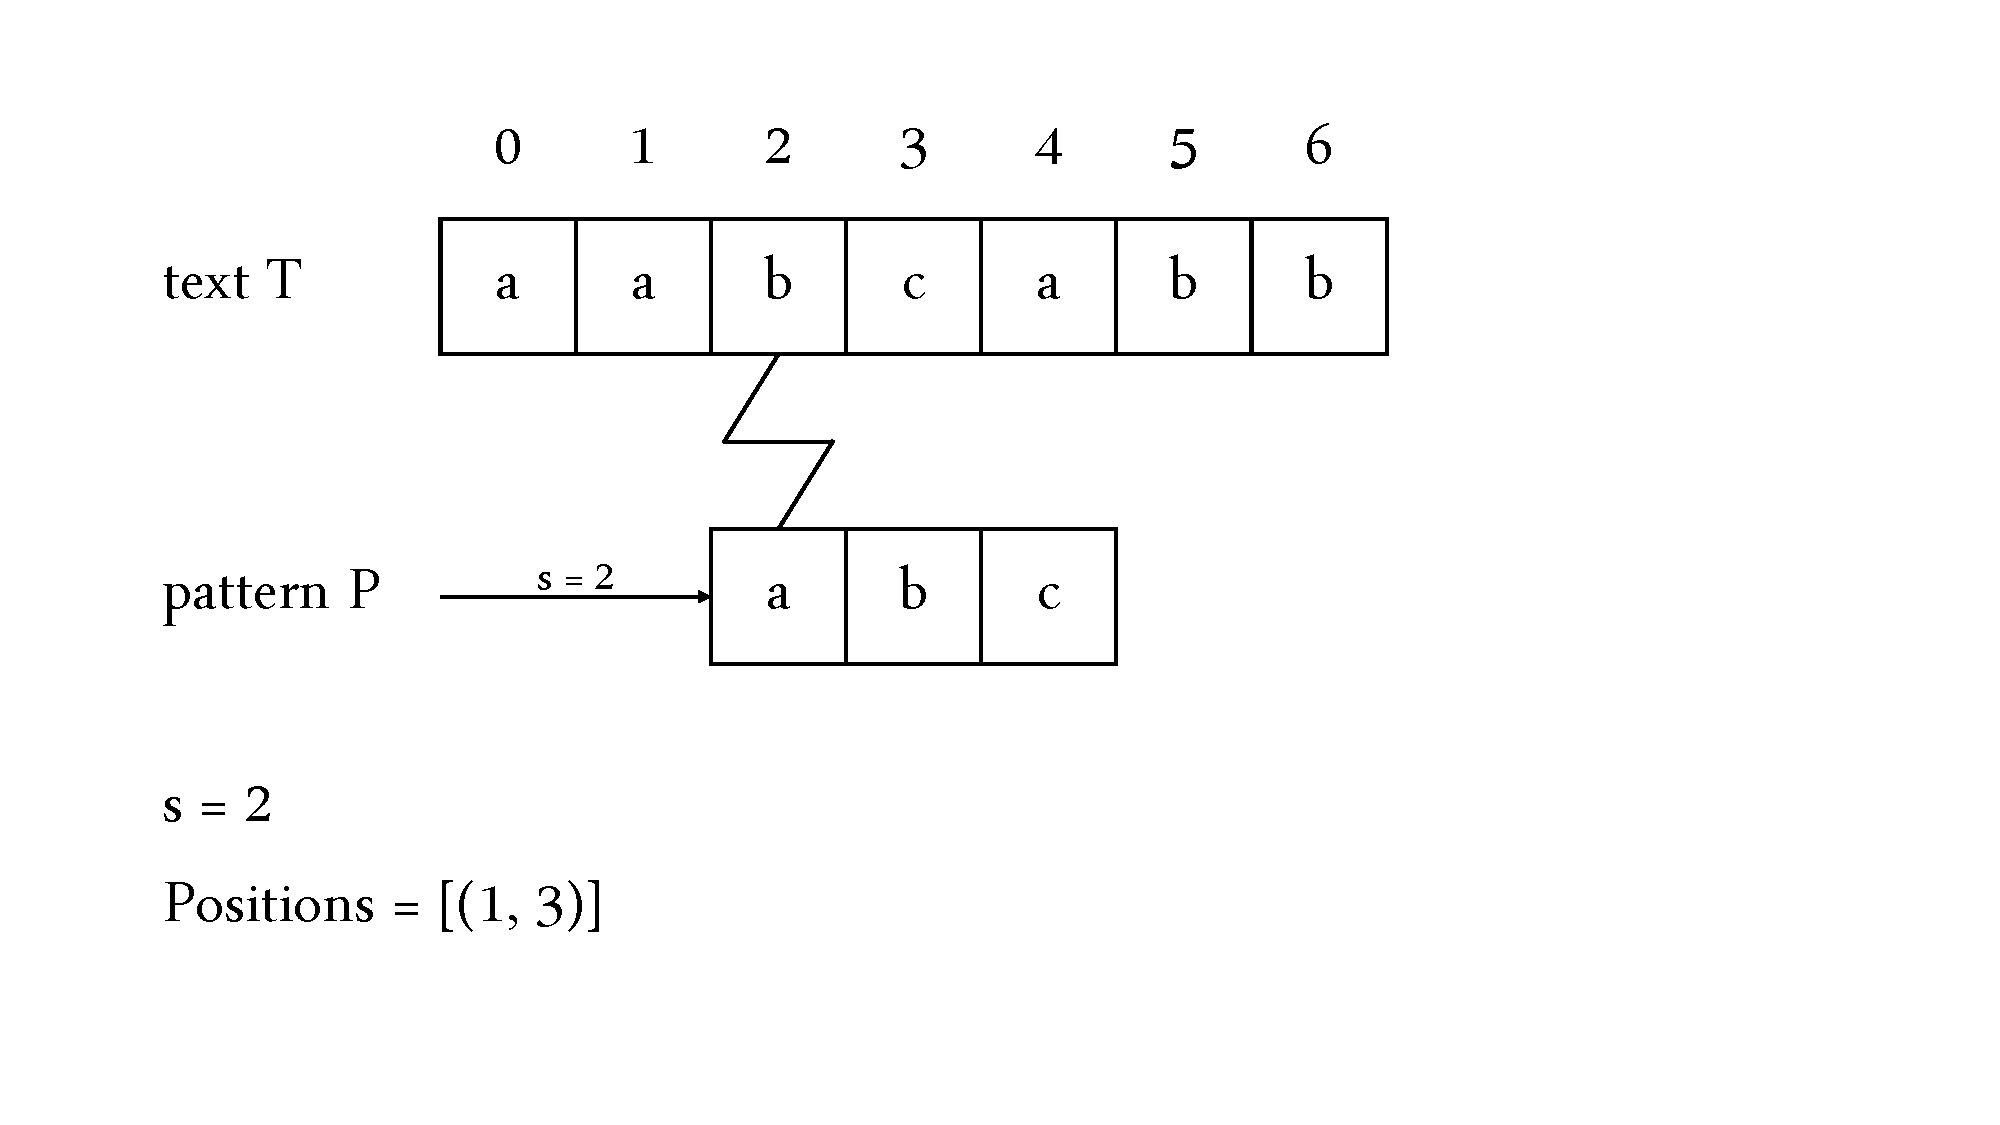
\includegraphics[width=0.8\textwidth, trim={2cm 2cm 5cm 2cm}, clip]{data/Illustrations/brute-force3.pdf}
            \caption{Step 3}
        \end{figure}
        \item The first character in pattern $P$ ('a') does not match the character in text $T$ ('b') at the current shift position $s = 2$.
        
        Skip to the next shift without updating $Positions$.

        \begin{figure}[H]
            \centering
            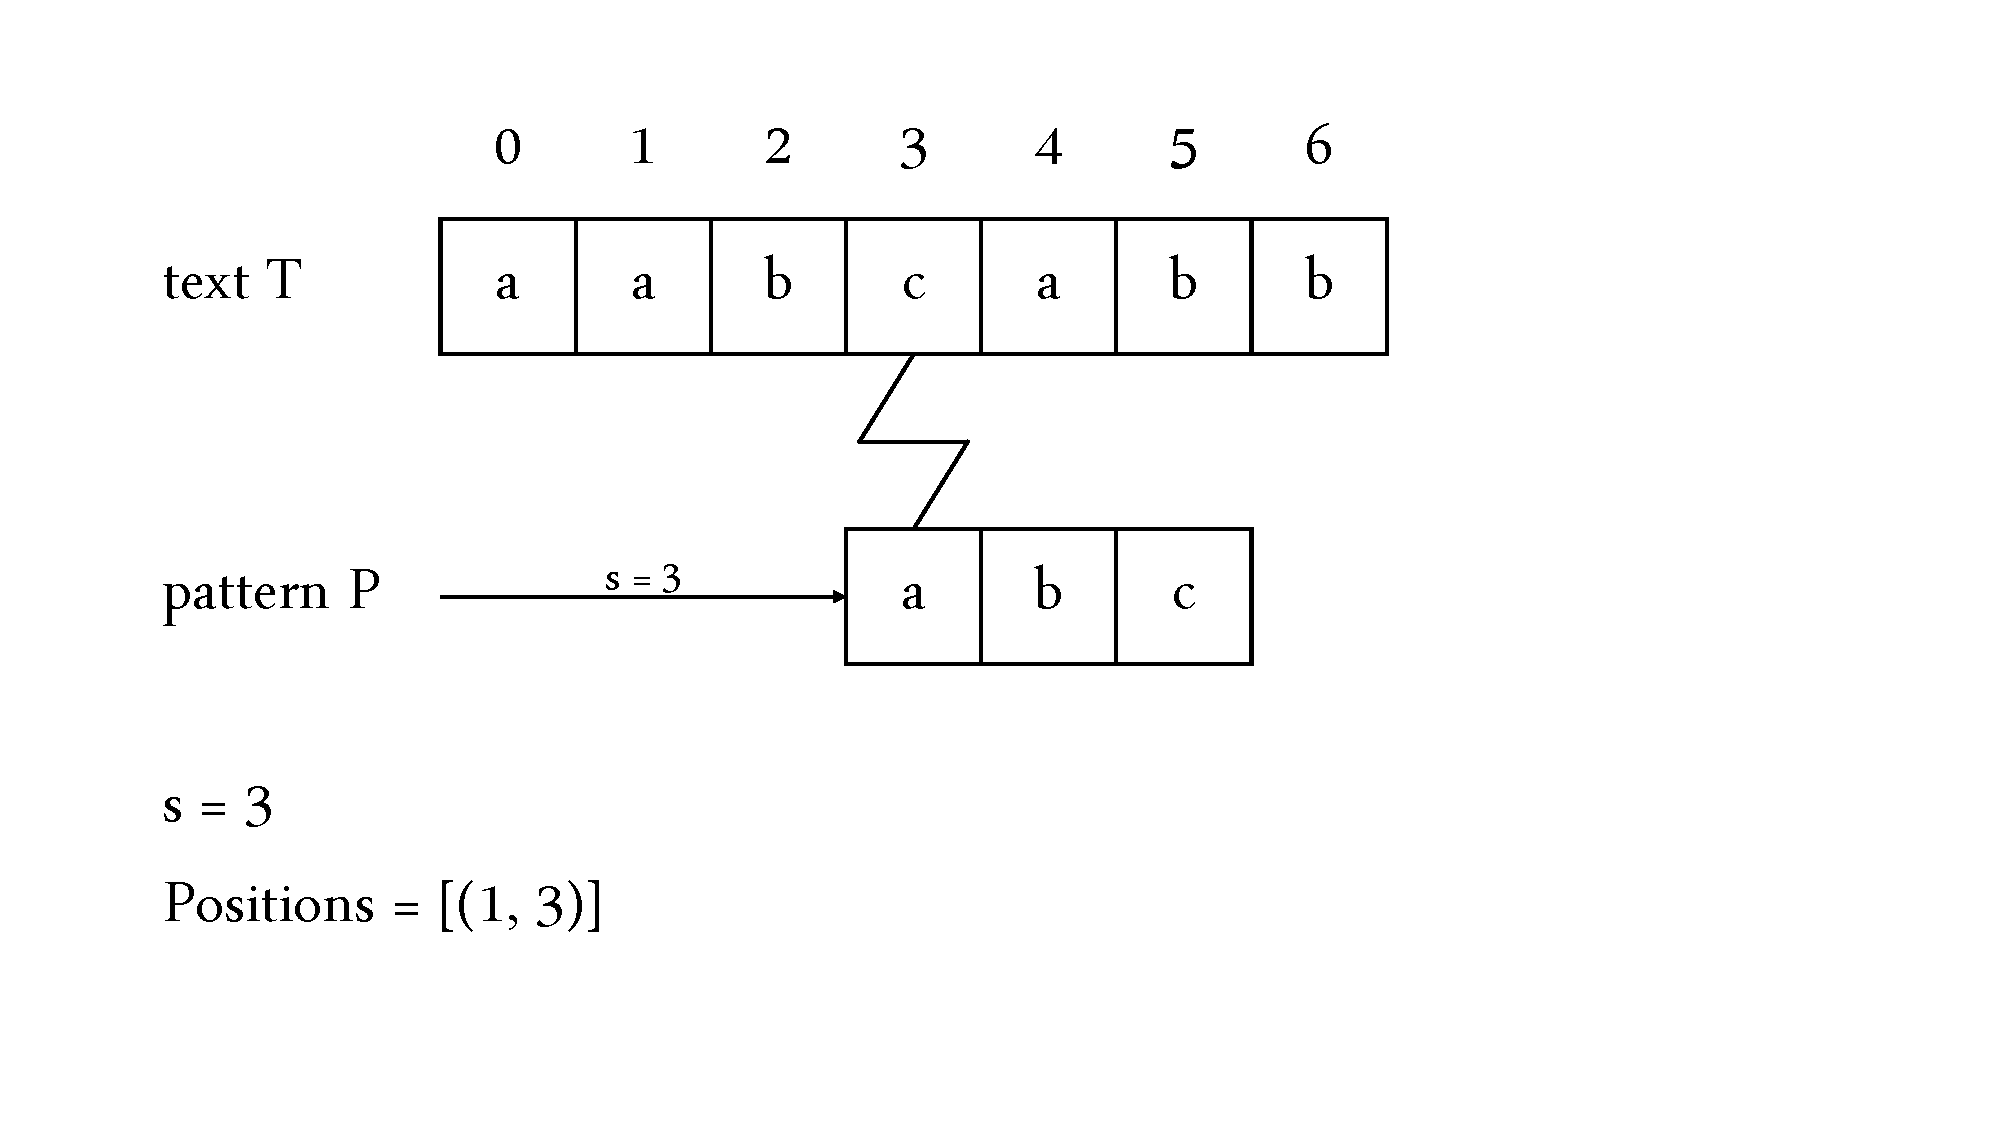
\includegraphics[width=0.8\textwidth, trim={2cm 2cm 5cm 2cm}, clip]{data/Illustrations/brute-force4.pdf}
            \caption{Step 4}
        \end{figure}
        \item The first character in pattern $P$ ('a') does not match the character in text $T$ ('c') at the current shift position $s = 2$.
        
        Skip to the next shift without updating $Positions$.

        \begin{figure}[H]
            \centering
            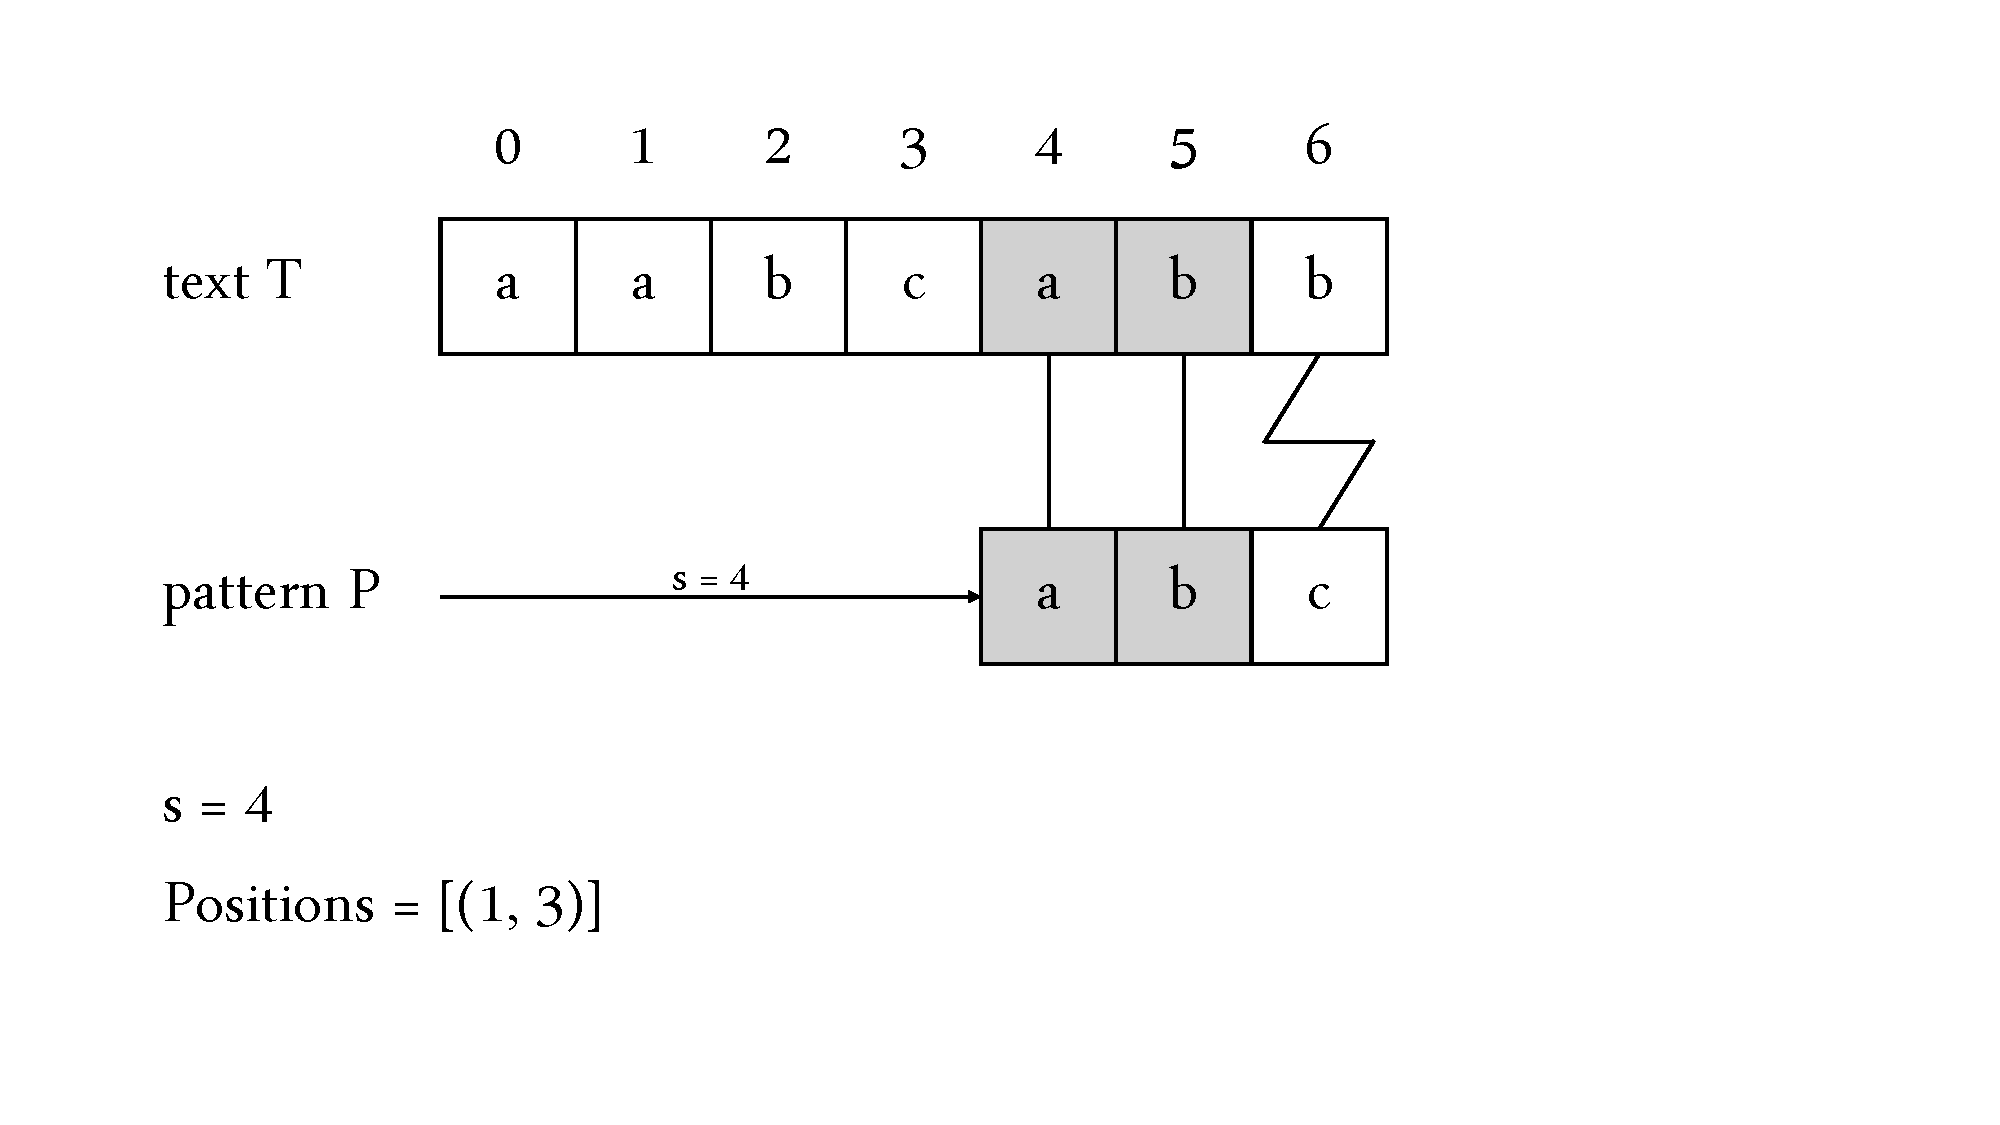
\includegraphics[width=0.8\textwidth, trim={2cm 2cm 5cm 2cm}, clip]{data/Illustrations/brute-force5.pdf}
            \caption{Step 5}
        \end{figure}

        \item The first two characters in pattern $P$ ('a', 'b') match the corresponding characters in text $T$,
        but the third character in pattern $P$ ('c') does not match the character in text $T$ ('b') at the current shift position $s = 4$.

        Skip to the next shift without updating $Positions$.

        \item After that, $s$ increases by 1. Because $s = 5$ and $n - m = 7 - 3 = 4$, we have $s > n - m$. The algorithm terminates and returns the list of found matches: $\text{Positions} = [(1, 3)]$.
    \end{itemize}
    

    \subsubsection{Complexity}
        \begin{table}[H]
        \centering
        \renewcommand{\arraystretch}{1.5}
        \begin{tabular}{|l|c|p{8cm}|}
        \hline
        \textbf{Metric} & \textbf{Complexity} & \textbf{Reasoning} \\ \hline
        \textbf{Time (Worst)} & $O(K \cdot m \cdot R \cdot C)$ & Occurs when patterns and text share many prefix characters (e.g., all 'A's). \\ \hline
        \textbf{Time (Average)} & $O(K \cdot R \cdot C)$ & In practice, a mismatch usually occurs after only a few character comparisons. \\ \hline
        \textbf{Time (Best)} & $O(K \cdot R \cdot C)$ & The first character of the pattern always results in a mismatch at every shift. \\ \hline
        \textbf{Auxiliary Space} & $O(1)$ & The algorithm uses only a constant amount of extra memory for loop indices. \\ \hline
        \end{tabular}
        \caption{Complexity Analysis of 2D Brute Force Algorithm}
        \end{table}

    \subsubsection{Discussion}
    \begin{itemize}
        \item In scenarios 1, the number of patterns $K$ is small, and the text is from $10 \times 10$ to $500 \times500$.
        Brute-force approach is efficient and likely linear running time $O(R \cdot C)$.
        \item In scenarios 2, the number of patterns $K$ is large, and the text is fixed at $100 \times 100$.
        This scenario is more challenging for the brute-force approach, as the running time multiplies by $K$ times,
        which is much longer compared to scenario 1.
        \item In conclusion, the brute-force approach is more suitable for scenarios with a small number of patterns.
        It is worse for scenarios with a large number of one.
    \end{itemize}
        